% Source of every NJU-Beamer runtime graphic. Each tikzpicture becomes one
% page; scripts/build-assets.sh splits the pages into shared-assets/ in the
% order listed there. Emblem, calligraphic name, English name and motto
% curves come from the njuvisual package (NJU LUG, LPPL 1.3c). The North
% Building, cedar and ribbon artwork below are original drawings of this
% project.
\documentclass[tikz,border=0pt]{standalone}
\usepackage{njuvisual}
\definecolor{NJUPurple}{HTML}{5C0F56}

% Cedar from the emblem: trunk plus four tiers; #1 x, #2 base y, #3 scale.
\newcommand{\NJUcedar}[3]{%
  \begin{scope}[shift={(#1,#2)},scale=#3]
    \fill (-0.35,0) rectangle (0.35,1.2);
    \fill (-3.2,1.2) -- (3.2,1.2) -- (0,4.4) -- cycle;
    \fill (-2.6,3.4) -- (2.6,3.4) -- (0,6.4) -- cycle;
    \fill (-2.0,5.5) -- (2.0,5.5) -- (0,8.3) -- cycle;
    \fill (-1.3,7.4) -- (1.3,7.4) -- (0,10.0) -- cycle;
  \end{scope}}

% One two-storey wing whose west end is at x=#1: body with window and
% string-course cutouts, roof with dormer-window cutouts, three dormers.
% #2 is the roof outline, which differs between the west and east wing.
\newcommand{\NJUwing}[2]{%
  \fill[even odd rule] (#1,0) rectangle (#1+17,7.2)
    \foreach \i in {0,...,6} {
      (#1+1.3+\i*2.3,1.1) rectangle (#1+2.4+\i*2.3,3.0)
      (#1+1.3+\i*2.3,4.3) rectangle (#1+2.4+\i*2.3,6.2)}
    (#1,3.65) rectangle (#1+17,3.85);
  \fill[even odd rule] #2
    \foreach \x in {3.5,8,12.5} {(#1+\x-0.45,9.9) rectangle (#1+\x+0.45,10.6)};
  \foreach \x in {3.5,8,12.5} {
    \fill[even odd rule] (#1+\x-1,9.6) rectangle (#1+\x+1,11.4)
      (#1+\x-0.45,9.9) rectangle (#1+\x+0.45,11.0);
    \fill (#1+\x-1.4,11.3) -- (#1+\x+1.4,11.3) -- (#1+\x,12.6) -- cycle;}}

% North Building, Gulou campus: two wings and a five-storey tower under a
% cross-ridge hip-and-gable roof. Units are mm, origin at the west end of
% the ground line. Windows are true cutouts (even-odd), so the silhouette
% can sit on any field in a single ink.
\newcommand{\NJUnorthbuilding}{%
  \NJUwing{0}{(-1.2,7.6) .. controls (-0.6,7.1) .. (0,7.1) -- (17,7.1) -- (17,10.6) -- (2.6,10.6) -- cycle}
  \NJUwing{29}{(47.2,7.6) .. controls (46.6,7.1) .. (46,7.1) -- (29,7.1) -- (29,10.6) -- (43.4,10.6) -- cycle}
  \fill[even odd rule] (17,0) rectangle (29,21.0)
    (21.4,0) -- (21.4,3.0) arc[start angle=180,end angle=0,radius=1.6] -- (24.6,0) -- cycle
    (18.3,1.1) rectangle (19.6,3.0) (26.4,1.1) rectangle (27.7,3.0)
    \foreach \y in {8.7,11.9,15.1} {
      (18.6,\y) rectangle (20.0,\y+2.0) (22.3,\y) rectangle (23.7,\y+2.0) (26.0,\y) rectangle (27.4,\y+2.0)}
    (19.2,18.2) rectangle (20.4,19.8) (21.0,18.2) rectangle (22.4,19.8)
    (23.6,18.2) rectangle (25.0,19.8) (25.6,18.2) rectangle (26.8,19.8);
  \fill (16.6,6.8) rectangle (29.4,7.6);
  \fill (16.6,20.6) rectangle (29.4,21.4);
  \fill (14.6,22.6) .. controls (15.6,21.5) .. (17.2,21.4) -- (28.8,21.4)
    .. controls (30.4,21.5) .. (31.4,22.6) -- (27.6,24.6) -- (18.4,24.6) -- cycle;
  \fill (16.9,25.2) .. controls (17.5,24.4) .. (18.6,24.3) -- (27.4,24.3)
    .. controls (28.5,24.4) .. (29.1,25.2) -- (26.4,25.6) -- (19.6,25.6) -- cycle;
  \fill[even odd rule] (18.4,24.5) -- (27.6,24.5) -- (23,28.4) -- cycle
    (21.8,25.9) -- (24.2,25.9) -- (23,27.3) -- cycle;
  \fill (22.75,28.0) rectangle (23.25,29.6);}

% Skyline: cedars flanking the North Building, 72.4 x 29.6 mm before scaling.
\newcommand{\NJUskyline}{%
  \NJUcedar{4.2}{0}{1.05}
  \NJUcedar{9.4}{0}{0.78}
  \begin{scope}[shift={(13,0)}]\NJUnorthbuilding\end{scope}
  \NJUcedar{63.4}{0}{0.9}
  \NJUcedar{68.6}{0}{0.68}}

% Lockup: emblem, calligraphic name and English name. #1 ink, #2 the color
% of the emblem's inner details (the field the lockup sits on).
\newcommand{\NJUlockup}[2]{%
  \node[anchor=north west,inner sep=0pt] (emb) at (0,0)
    {\njuemblem[color=#1,color*=#2]{!}{12.2mm}};
  \node[anchor=north west,inner sep=0pt] (zh) at ([xshift=2.6mm,yshift=-1.0mm]emb.north east)
    {\njuname[#1]{29mm}{!}};
  \node[anchor=north west,inner sep=0pt] at ([yshift=-1.6mm]zh.south west)
    {\njuname*[#1]{29mm}{!}};}

\begin{document}
% 1 Slide background, 160 x 90 mm (beamer aspectratio=169). The skyline and
% motto stay inside the bottom 10 mm band that the theme's footline reserves
% (only the tower roof rises above it, left of the text margin's first cm).
\begin{tikzpicture}[x=1mm,y=1mm]
  \path[use as bounding box] (0,0) rectangle (160,90);
  \fill[NJUPurple] (0,0) rectangle (160,0.55);
  \begin{scope}[shift={(2.2,0.55)},scale=0.40,fill=NJUPurple]\NJUskyline\end{scope}
  \begin{scope}[shift={(120.6,86.2)},scale=0.82,transform shape]\NJUlockup{NJUPurple}{white}\end{scope}
  \node[anchor=south east,inner sep=0pt] at (156.5,1.9) {\njumotto[NJUPurple]{!}{6.4mm}};
\end{tikzpicture}
% 2 Emblem, purple on light fields.
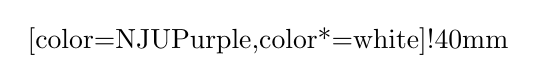
\begin{tikzpicture}
  \node[inner sep=0pt] {\njuemblem[color=NJUPurple,color*=white]{!}{40mm}};
\end{tikzpicture}
% 3 Emblem, white on purple fields.
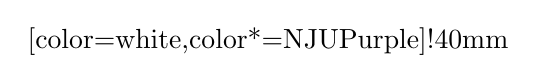
\begin{tikzpicture}
  \node[inner sep=0pt] {\njuemblem[color=white,color*=NJUPurple]{!}{40mm}};
\end{tikzpicture}
% 4 Lockup, purple.
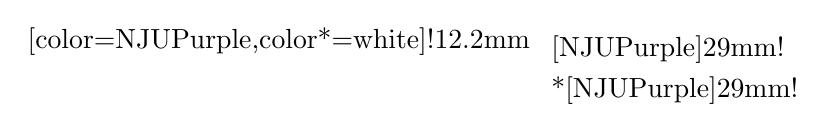
\begin{tikzpicture}[x=1mm,y=1mm]\NJUlockup{NJUPurple}{white}\end{tikzpicture}
% 5 Lockup, white on purple.
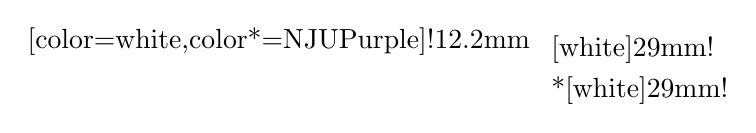
\begin{tikzpicture}[x=1mm,y=1mm]\NJUlockup{white}{NJUPurple}\end{tikzpicture}
% 6 Skyline, purple.

\begin{tikzpicture}[x=1mm,y=1mm,fill=NJUPurple]\NJUskyline\end{tikzpicture}
% 7 Skyline, white.
\begin{tikzpicture}[x=1mm,y=1mm,fill=white]\NJUskyline\end{tikzpicture}
% 8 Motto, purple.

\begin{tikzpicture}\node[inner sep=0pt] {\njumotto[NJUPurple]{!}{20mm}};\end{tikzpicture}
% 9 Motto, white.

\begin{tikzpicture}\node[inner sep=0pt] {\njumotto[white]{!}{20mm}};\end{tikzpicture}
% 10 Ribbons: translucent white curves for dark gradient fields, 160 x 90 mm.
\begin{tikzpicture}[x=1mm,y=1mm]
  \path[use as bounding box] (0,0) rectangle (160,90);
  \clip (0,0) rectangle (160,90);
  \foreach \i in {0,...,44} {
    \pgfmathsetmacro{\o}{0.04+0.20*abs(sin(\i*9))}
    \draw[white,opacity=\o,line width=0.16pt]
      plot[domain=-4:164,samples=90,smooth]
      (\x,{8+\i*0.75+(9+\i*0.42)*sin(\x*1.35+\i*3.2)+(3+\i*0.12)*sin(\x*0.55-\i*5.5)});}
\end{tikzpicture}
\end{document}
